
\documentclass[12pt]{article}
\usepackage[margin=1in]{geometry}
\usepackage[pdftex]{graphicx}
\usepackage{multirow}
\usepackage{setspace}
\usepackage{enumitem}
\pagestyle{plain}
\setlength\parindent{0pt}

\begin{document}

% Course information
\begin{tabular*}{\textwidth}{l @{\extracolsep{\fill}} r}
  & \multirow{3}{*}{
\includegraphics[height=1.0in]{logo.jpg}} \\
  \large Computers in Physics Exps. & \\
  \large Spring Quarter 2020 & \\
  \large Physics 116C & \\
\end{tabular*}
\vspace{10mm}


% Professor information
\begin{tabular}{ l l }
  \multirow{6}{*}{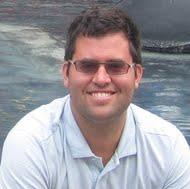
\includegraphics[height=1.25in]{mike.jpg}} & \\
  & \\
  & \large Michael Mulhearn \\
  & \large mulhearn@physics.ucdavis.edu \\
  & \large Physics 317 \\
  & \\
\end{tabular}
\vskip 0.5cm
\noindent
\begin{tabbing}
\hspace*{9em}\= \hspace*{10em} \= \hspace*{6em} \= \kill % set the tabbings
\textbf {Lectures:} \> MWF  1:10-2:00 PM \> 140 Physics (Cancelled!)\\
%\> \> 152 Roessler \> (F) \\
\hspace*{9em}\= \hspace*{5em} \= \hspace*{8em} \= \kill % set the tabbings
\\
\textbf {Lab:}    \> Section 1: \>  M 4:10-7:00 PM \>152 Roessler (Cancelled!)\\
                        \> Section 2: \> W 3:10-6:00 PM \> 152 Roessler (Cancelled!)\\
\\
\hspace*{9em}\= \kill % set the tabbings
\textbf {References:}  \>  {\tt https://www.scipy-lectures.org} \\
\> Online lecture notes on data analysis. \\
\\
\textbf{Office Hours:} \> TBD \\
\textbf{Lab Instructor:} \> Rahim Ullah \\
\textbf{Final Exam:} \> No Final Exam \\
\end{tabbing}

\noindent
\textbf {COVID-19 Response:}
To facilitate shelter-in-place during the COVID-19 pandemic, and to
accommodate the diverse challenges that students are likely facing,
this course will be taught in an asynchronous fashion.  As much as
possible, there will be no pre-arranged times for activitates.  On an
approximately weekly timescale, new material will provided including
activities and assignments.  You should strive to finish the
assignments within two weeks, but deadlines will be flexible.  Try not
to get too far behind, however, or you will struggle to finish.

\noindent
\textbf {On-line Help Sessions:}
The instructor and TA will be available at specified times to offer
help.  More details will be provided soon.

\noindent
\textbf {Course Description:}
Modern experiments rely heavily on microprocessors to acquire and
analyze experimental data.  This course uses the Arduino
microprocessor as a platform for creating data acquisition systems in
different experimental contexts.  We will use Scientific Python for
analysis of experimental data.  Topics include statistical
distributions, experimental uncertainties, statistical analysis,
Fourier analysis, and noise.\\

\noindent
\textbf {Lab Safety:}
Even though you will not be attending lab, you should complete the
online course for Electrical Safety at \\ {\tt
  http://safetyservices.ucdavis.edu/training/electrical-safety}.\\

\begin{samepage}
\vskip 0.5cm
\noindent
\textbf {Course Outline}:

\begin{table}[h!]
\begin{tabular}{ lll }
\hline
\textbf{Week} & \textbf{Dates} & \textbf{Topics} \\
\hline
1 & 30 Mar,1,3 Apr & Cancelled \\
\hline
2 & 6,8,10 Apr & CPUs and Assembly  \\
\hline
3 & 13,15,17 Apr & Distributions \\
\hline
4 & 20,22,24 Apr &  \\
% F:  Fourier Analysis
\hline
5 & 27,29 Apr 1 May & \\
\hline
6 & 4,6,8 May & \\
\hline
7 & 11,13,15 May & \\
% F: 
\hline
8 & 18,20,22 May & \\
\hline
9 & (25),27,29 May &  \\
% F: 
\hline
10 & 1,3 Jun &  \\
% F: 
\hline
\end{tabular} 
\end{table}
\end{samepage}
\end{document}

